\documentclass[
../../EiKI_Summary.tex,
]
{subfiles}
    
\externaldocument[ext:]{../../EiKI_Summary.tex}
% Set Graphics Path, so pictures load correctly
\graphicspath{{../../}}

\begin{document}
\section{AI Systems}
\subsection{What is an AI System?}

\begin{defbox*}
    An AI System can be defined as the study of \defc{rational agents} and \defc{their environments}
\end{defbox*}

\begin{figure}
    [htp]
    \centering
    
\includegraphics[width=0.5\textwidth]{Pics/02/Agent_Environment.png}
\end{figure}

\subsubsection{Environment}
\begin{itemize}
    \item ''The surroundings or conditions in which a person, animal, or plant lives or operates'' - Oxford Dictionary
    \item In AI: The surrounding of an (AI) agent, where the agent operates
    \item Does not have to be real - Can be artificial
    \item Example: 
    \begin{itemize}
        \item Selfdriving cars: Street, traffic, weather, road signs, \dots
        \item Chess: Board, pieces,\dots
    \end{itemize}
\end{itemize}

\defc{Characteristics of Environments}

\begin{defbox}
    [Discrete vs. Continous]
    \defc{Discrete:} Environment has countable number of distinct, well defined states\\
    \defc{Continous:} Not discrete - Uncountable number of states
\end{defbox}

For Example: 
\begin{itemize}
    \item Discrete: Chess - Every state of the board is mathematically determinable and defined
    \item Continous: Selfdriving car - Practically infinite positions and conditions
\end{itemize}

\begin{defbox}
    [Observable vs. Partially Observable / Unobservable]
    \defc{Observable:} State is completely determinable at each point in time\\
    \defc{Partially Observable:} State is only partially determinable or only determinable at specific points in time\\
    \defc{Unobservable:} State is never determinable
\end{defbox}

\begin{defbox}
    [Static vs. Dynamic]
    \defc{Static:} Environment does \textbf{not} change while the agent is acting\\
    \defc{Dynamic:} Environment can change while the agent is acting
\end{defbox}

For Example:
\begin{itemize}
    \item Static: Jigsaw puzzle - State does not change without the agents action
    \item Dynamic: Driving - State still changes even when the agent stops acting
\end{itemize}

\begin{defbox}
    [Single Agent vs. Multiple Agents]
    \defc{Single Agent:} Environment contains only one agents\\
    \defc{Multiple Agents:} Environment can contain multiple agents
\end{defbox}

\begin{defbox}
    [Accessible vs. Inaccessible]
    \defc{Accessible:} Agent can obtain complete and accurate information about the state\\
    \defc{Inaccessible:} Agent cannot obtain complete or only inaccurate information
\end{defbox}

\begin{defbox}
    [Deterministic vs. Stochastic / Probabilistic]
    \defc{Deterministic:} Next state is completely determined by the current state and the actions of the agents\\
    \defc{Probabilistic:} Next state is also influenced by other factors
\end{defbox}

\begin{defbox}
    [Episodic vs. Non-episodic / Sequential]
    \defc{Episodic:} Each \textbf{episode} consists of the agent perceiving and then acting -  every action is dependent only on the episode\\
    \defc{Non-episodic:} Actions are also dependent on past memory
\end{defbox}

These characteristics are important, as the environment specifies the specific needs of the agent: 
\begin{itemize}
    \item Different environments require different agent designs
    \item Not every algorithm works for a specific environment
\end{itemize} 

\subsubsection{Agents}
\begin{itemize}
    \item \defc{Sense:} Perceives its environment
    \item \defc{Think:} Makes decisions autonomously
    \item \defc{Act:} Acts upon the environments
\end{itemize}

\begin{figure}
    [htp]
    \centering
    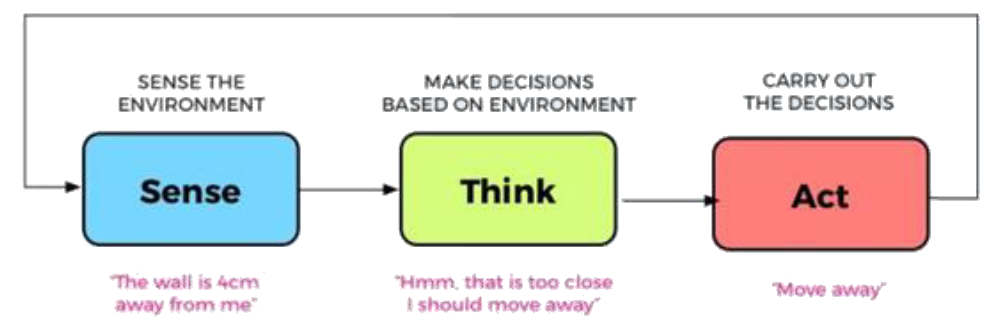
\includegraphics[width=0.5\textwidth]{Pics/02/Agent.png}
\end{figure}

\begin{defbox}
    [Rules of AI Agents]
    \begin{enumerate}
        \item Must be able to perceive its environment
        \item Observations must be used to make decisions
        \item Decisions should be used to act
        \item (Action should be rational)
    \end{enumerate}
\end{defbox}

\begin{defbox}
    [Rational Agents]
    Maximizes the performance and yield the best positive outcome. \\
    Performance is hereby often measured by a function that evaluates a sequence of actions. This function is task-dependent and cannot be generalized.
\end{defbox}

\subsubsection{Types of Agents}

\begin{defbox}
    [Reflex Agent]
    Act only on the basis of the current percept, ignores past memory
    \begin{itemize}
        \item Implemented through condition-action rules - map state to action
        \item Problem:
        \begin{itemize}
            \item Limited decision making
            \item No knowledge about anything that cannot be currently perceived
            \item Hard to handle in complex environments
        \end{itemize}
    \end{itemize}
    
    \begin{center}
        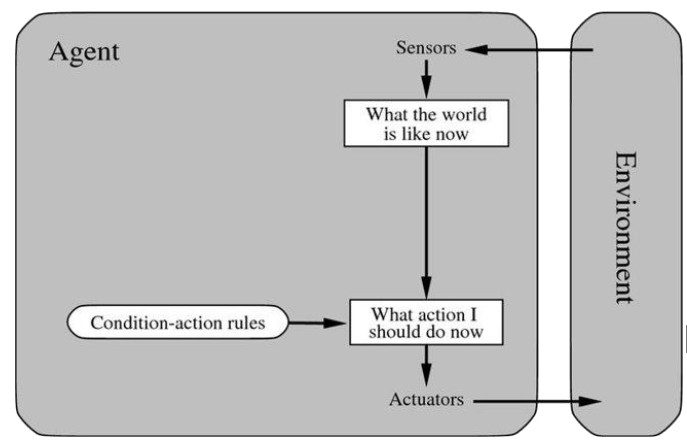
\includegraphics[width=0.5\textwidth]{Pics/02/ReflexAgent.png}
    \end{center}
\end{defbox}

\begin{defbox}
    [Model-Based Agent]
    Similar decision making to reflex agent, but keep track of the world state 
    \begin{itemize}
        \item Input is interpreted and mapped to an internal state representation of the world
        \item Problem: 
        \begin{itemize}
            \item How do these action affect the internal representation of the world?
            \item What details are needed for the world model?
        \end{itemize}
    \end{itemize}

    \begin{center}
        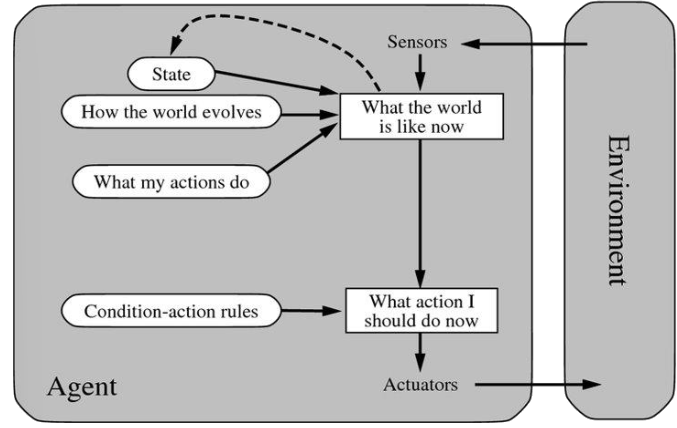
\includegraphics[width=0.5\textwidth]{Pics/02/ModelBasedAgent.png}
    \end{center}
\end{defbox}

\begin{defbox}
    [Goal-Based Agent]
    Essentially a Model-Based Agent with additional functionality that stores desirable states
    \begin{itemize}
        \item Knows what states are desirable and acts towards them
        \item Problem:
        \begin{itemize}
            \item Difficult to choose actions if a lot of actions are required to achieve a goal
        \end{itemize}
    \end{itemize}

    \begin{center}
        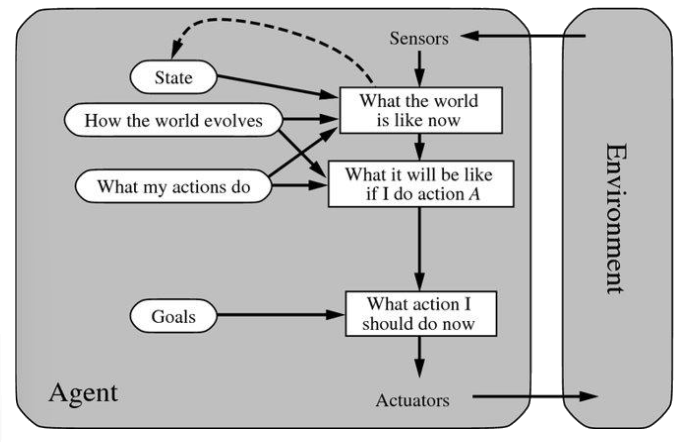
\includegraphics[width=0.5\textwidth]{Pics/02/GoalBasedAgent.png}
    \end{center}
\end{defbox}

\begin{defbox}
    [Utility-Based Agent]
    Similar to Goal-Based Agents, but instead of providing goals it provides a utility function for rating actions and scenarios based on the desirability of the result
    \begin{itemize}
        \item Goals provide binary distinction, while utility functions provide a continuous measure of desirability
        \item Can handle selection between two conflicting goals - ''Speed or safety''
    \end{itemize}

    \begin{center}
        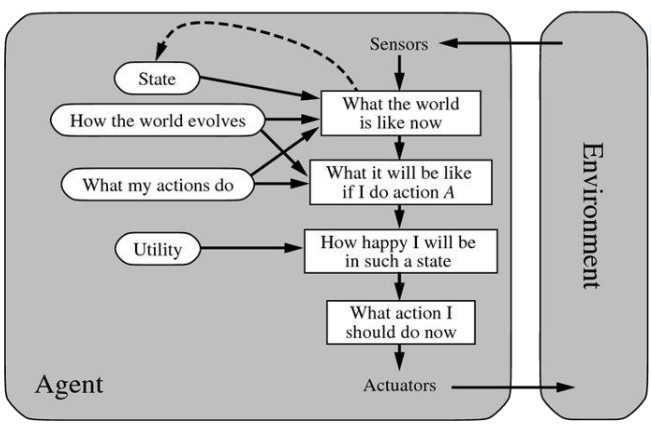
\includegraphics[width=0.5\textwidth]{Pics/02/UtilityBasedAgent.png}
    \end{center}
\end{defbox}

\begin{defbox}
    [Learning Agent]
    Employs additional learning element to gradually improve and become more knowledgable over time about an environment
    \begin{itemize}
        \item Can learn from past experiences
        \item Is more robust towards unknown environments
        \item A learning agent has four conceptual components:
        \begin{enumerate}
            \item \defc{Learning Element:} Makes improvements by learning from the environment
            \item \defc{Critic:} Gives feedback on the performance of the agent according to a fixed metric
            \item \defc{Performance Element:} Selects the best action according to the critic
            \item \defc{Problem Generator:} Responsible for suggesting actions that will lead to new experiences
        \end{enumerate}
    \end{itemize}

    \begin{center}
        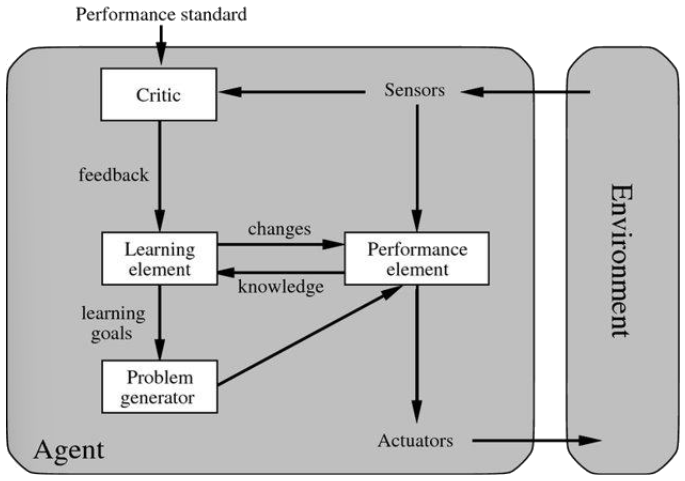
\includegraphics[width=0.5\textwidth]{Pics/02/LearningAgent.png}
    \end{center}
\end{defbox}

\subsection{Creating Intelligent Agents}

\subsubsection{Search Algorithms}
Define ''finding a good action'' as a search problem and use search algorithm to solve it. Most of these seach algorithms are tree based, altough Bread-First is used often.

\subsubsection{Reinforcement Learning}
Developed in psychology, Reinforcement Learning essentially is a process of trial and error - Try something out, have a reaction to it, learn wether it was good or bad. Reactions or actions are based on out observations or experiences.

\begin{figure}
    [htp]
    \centering
    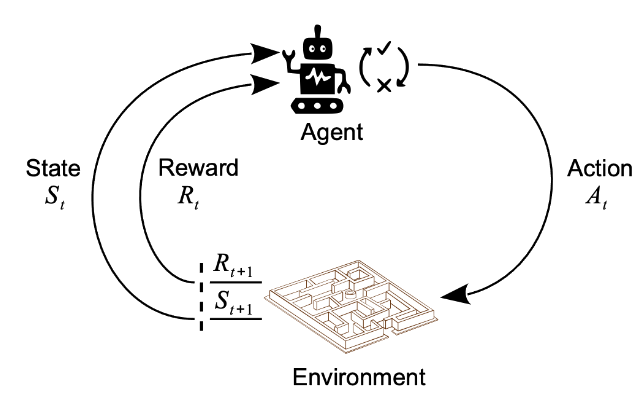
\includegraphics[width=0.5\textwidth]{Pics/02/ReinforcementLearningLoop.png}
\end{figure}

\newpage
\subsubsection{Genetic Algorithms}
Inspired by Darwins ''Theory of natural selection'', this model build multiple different agents and evaluates every one of them. The agent with the highest performance is selected and new models are built based on it. This is done until the performance is good enough.

\begin{figure}
    [htp]
    \centering
    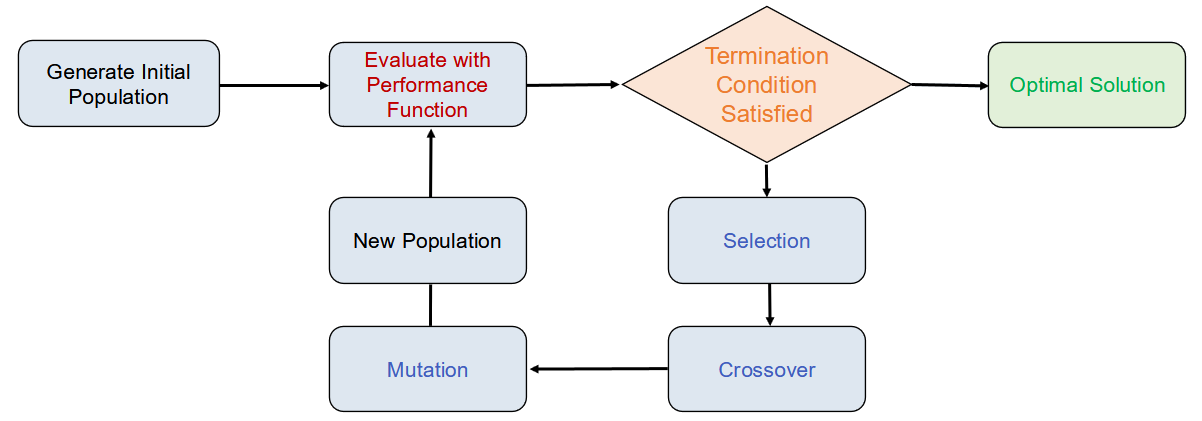
\includegraphics[width=0.5\textwidth]{Pics/02/GeneticAlgorithms.png}
\end{figure}


\end{document}